\documentclass[../chapter_2.tex]{subfiles}
\addbibresource{../../Thesis.bib}

\begin{document}
Although not calculated often, the modeling of the aircraft's landing gear are important and should not be overlooked. However, because of the flight paths investigated in this thesis focus solely on the aircraft during flight, a simplified dynamic model is used to describe the forces and moments acting on the landing gear during landing. It should be noted that the aerodynamic calculations of the landing gear occur in the aerodynamically modeling section, while this section focuses on the moments and forces generated from the runway opposing the weight of the aircraft.

To describe the forces and moments generated during landing, a mass-spring damper system (Figure \ref{fig:ldgfbd}) can be used in simulate the the struts, levers, and tire depression (Figure \ref{fig:ldg}) that absorb much of the forces, moments and vibrations that act onto the aircraft during landing.

\begin{figure}[!h]
        \centering
    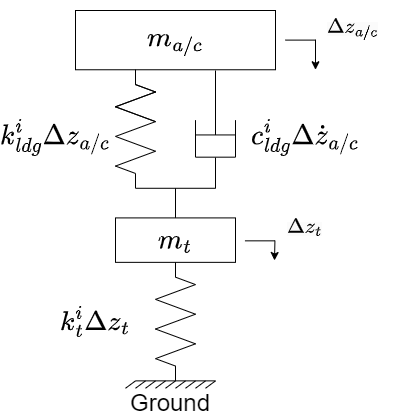
\includegraphics[width=.4\linewidth]{../../Figures/ldgfbd.drawio.png}
    \caption{Mass-spring damper system, representing the components of landing gear on the aircraft (adapted from \cite{xingStrengthAnalysisDiagonal2012}).}
    \label{fig:ldgfbd}
\end{figure}

\begin{figure}[!h]
        \centering
    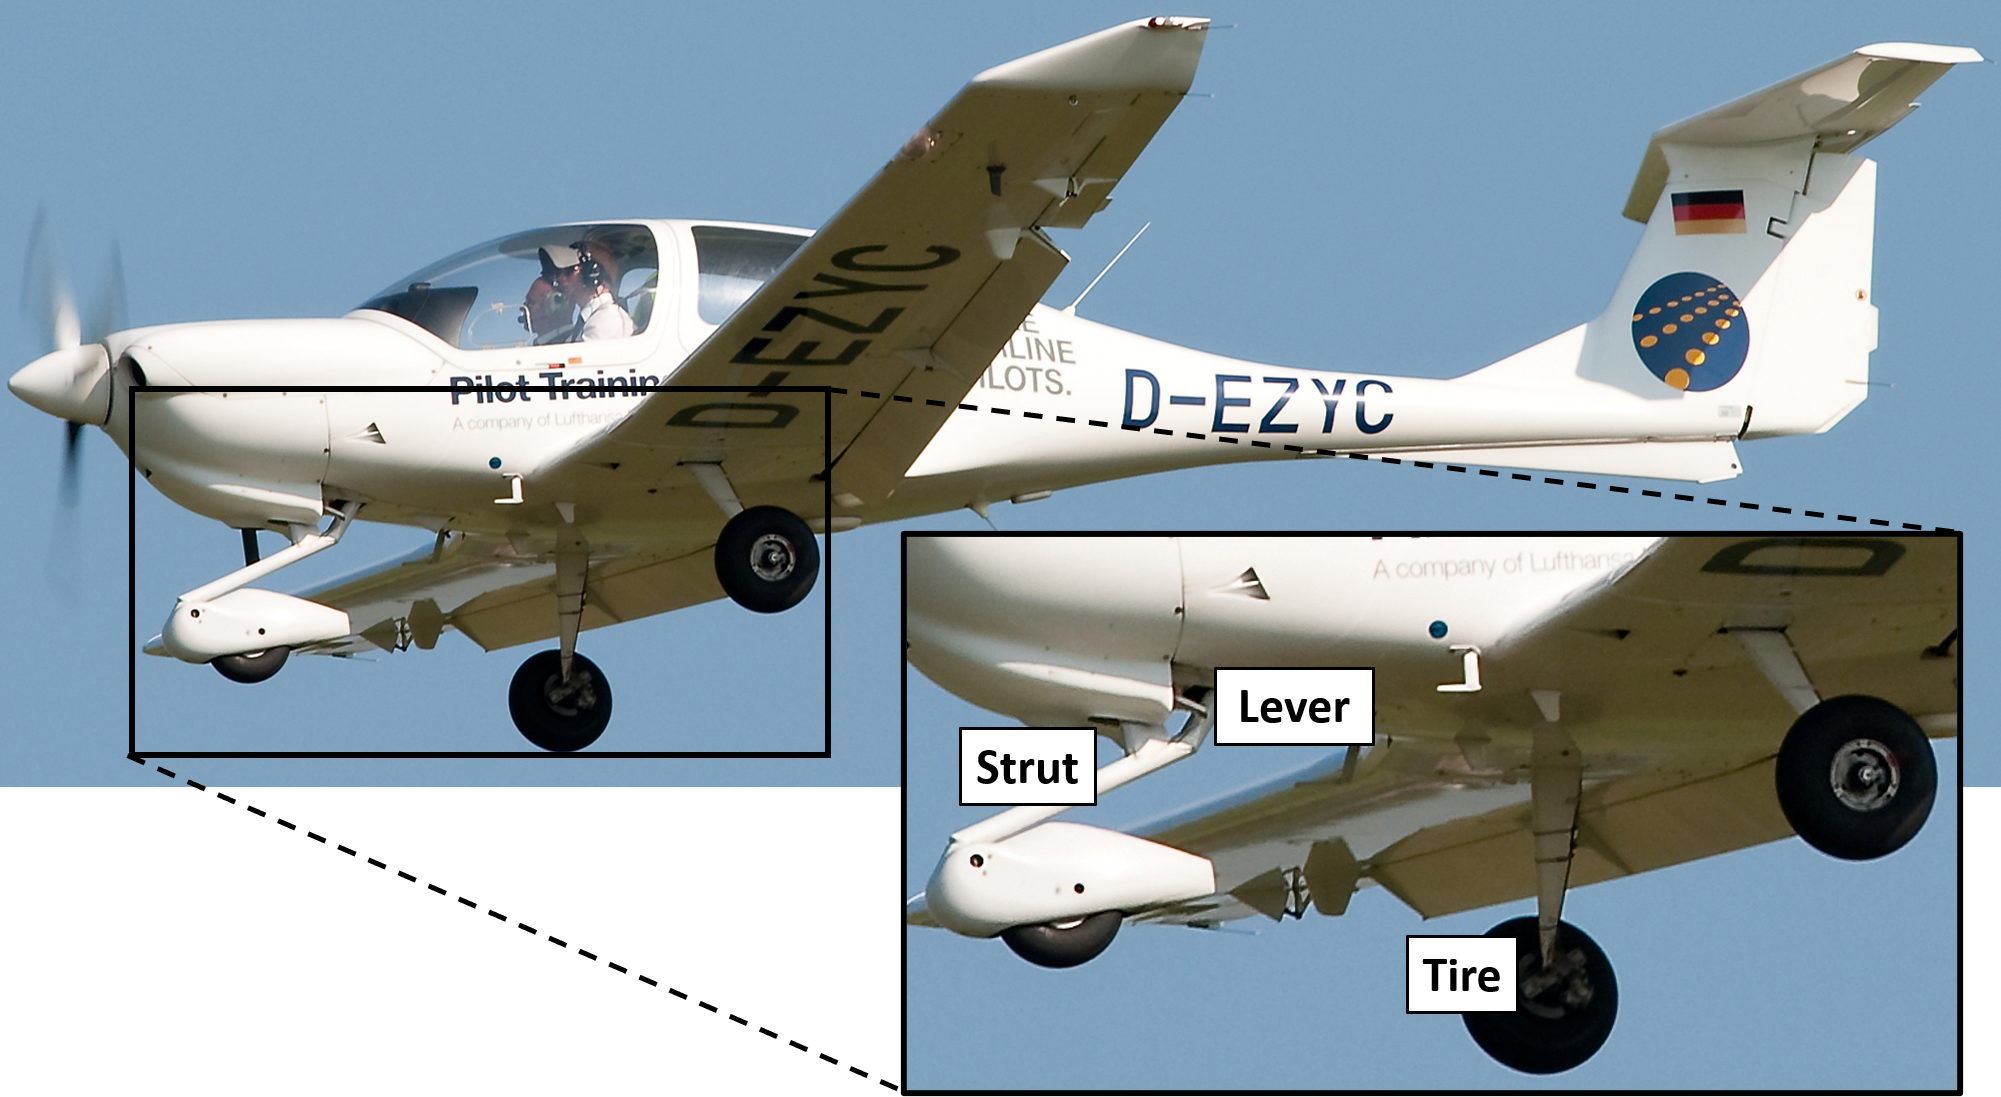
\includegraphics[width=.75\linewidth]{../../Figures/LandingGear.png}
    \caption{Identification of the landing gear components on the Diamond DA40.}
    \label{fig:ldg}
\end{figure}

Expanding Newton's second law, the forces on each landing gear are solved in the vertical direction (Equation \ref{eq:ldgforces})

\begin{equation}
    \sum F^i_z = m\,a_z = k^i_t\, \Delta z_t\, + \, k^i_{ldg}\, \Delta z_{a/c}\, + c^i_{ldg}\, \Delta \dot{z}_t,
    \label{eq:ldgforces}
\end{equation}

where $k^i_{ldg}$ and $c^i_{ldg}$ are the spring and damper coefficients of the struts and levers respectively (see Table \ref{tbl:ldgcoeff} for the values used in this simulated model). $\Delta z_{a/c}$ and $\Delta \dot{z}_t$, are the deflection and rate of deflection of the aircraft during landing. $k^i_t$ and $\Delta z_t$ are the tire 'spring' coefficient and tire depression respectively. For a general aviation aircraft, the depression of the tire upon landing is relatively small such that this term is thrown out.  

\begin{table}[!ht]
    \caption{List of spring and damper coefficients for nose and rear landing gear.}
    \label{tbl:ldgcoeff}
    \centering
\begin{tabular}{|c|c|c|c|}
    \hline
    &&&\\
\textbf{i} & \textbf{Landing Gear Location} & \textbf{Spring Coefficient}, $k\,\left[\frac{N}{m}\right]$ & \textbf{Damper Coefficient}, $c\,\left[\frac{N\,s}{m}\right]$ \\
&&&\\
\hline
1 & Nose                  & $50,000$                & $11,300$               \\
\hline
2 & Rear Right            & $80,000$                & $14,300$               \\
\hline
3 & Rear Left             & $80,000$                & $14,300$               \\
\hline
\end{tabular}
\end{table}

The observed moments are solved by taking the cross product between the calculated forces of each landing gear and the moment arm (Equation \ref{eq:ldgmoments}).

\begin{equation}
    \sum M^i = \textnormal{cross}([\,0\,;\,0\,;\,F^i_z\,],[\,x^i\,;\,y^i\,;\,z^i\,])
    \label{eq:ldgmoments}
\end{equation}

In Equation \ref{eq:ldgmoments}, $x^i$, $y^i$, and $z^i$ represent the moment arm that is derived from the center of gravity for the aircraft down to where each tire makes contact with the ground.

As a final note, it should be made clear that the forces and moments that act upon the landing gear if and only if a tire has made contact with the ground, for computational efficiency.

\end{document}